% Created 2025-10-15 on 11:59
% Intended LaTeX compiler: pdflatex
\documentclass[12pt]{article}

%%%% settings when exporting code %%%% 

\usepackage{listings}
\lstdefinestyle{code-small}{
backgroundcolor=\color{white}, % background color for the code block
basicstyle=\ttfamily\small, % font used to display the code
commentstyle=\color[rgb]{0.5,0,0.5}, % color used to display comments in the code
keywordstyle=\color{black}, % color used to highlight certain words in the code
numberstyle=\ttfamily\tiny\color{gray}, % color used to display the line numbers
rulecolor=\color{black}, % color of the frame
stringstyle=\color[rgb]{0,.5,0},  % color used to display strings in the code
breakatwhitespace=false, % sets if automatic breaks should only happen at whitespace
breaklines=true, % sets automatic line breaking
columns=fullflexible,
frame=single, % adds a frame around the code (non,leftline,topline,bottomline,lines,single,shadowbox)
keepspaces=true, % % keeps spaces in text, useful for keeping indentation of code
literate={~}{$\sim$}{1}, % symbol properly display via latex
numbers=none, % where to put the line-numbers; possible values are (none, left, right)
numbersep=10pt, % how far the line-numbers are from the code
showspaces=false,
showstringspaces=false,
stepnumber=1, % the step between two line-numbers. If it's 1, each line will be numbered
tabsize=1,
xleftmargin=0cm,
emph={anova,apply,class,coef,colnames,colNames,colSums,dim,dcast,for,ggplot,head,if,ifelse,is.na,lapply,list.files,library,logLik,melt,plot,require,rowSums,sapply,setcolorder,setkey,str,summary,tapply},
aboveskip = \medskipamount, % define the space above displayed listings.
belowskip = \medskipamount, % define the space above displayed listings.
lineskip = 0pt} % specifies additional space between lines in listings
\lstset{style=code-small}
%%%% packages %%%%%

\usepackage[utf8]{inputenc}
\usepackage[T1]{fontenc}
\usepackage{lmodern}
\usepackage{textcomp}
\usepackage{color}
\usepackage{graphicx}
\usepackage{grffile}
\usepackage{wrapfig}
\usepackage{rotating}
\usepackage{longtable}
\usepackage{multirow}
\usepackage{multicol}
\usepackage{changes}
\usepackage{pdflscape}
\usepackage{geometry}
\usepackage[normalem]{ulem}
\usepackage{amssymb}
\usepackage{amsmath}
\usepackage{amsfonts}
\usepackage{dsfont}
\usepackage{array}
\usepackage{ifthen}
\usepackage{hyperref}
\usepackage{natbib}
\RequirePackage{setspace} % to modify the space between lines - incompatible with footnote in beamer
\renewcommand{\baselinestretch}{1.1}
\geometry{a4paper, left=10mm, right=10mm, top=10mm}
\usepackage{titlesec}
\usepackage{etoolbox}

\makeatletter
\patchcmd{\ttlh@hang}{\parindent\z@}{\parindent\z@\leavevmode}{}{}
\patchcmd{\ttlh@hang}{\noindent}{}{}{}
\makeatother
\RequirePackage{colortbl} % arrayrulecolor to mix colors
\definecolor{myorange}{rgb}{1,0.2,0}
\definecolor{mypurple}{rgb}{0.7,0,8}
\definecolor{mycyan}{rgb}{0,0.6,0.6}
\newcommand{\lightblue}{blue!50!white}
\newcommand{\darkblue}{blue!80!black}
\newcommand{\darkgreen}{green!50!black}
\newcommand{\darkred}{red!50!black}
\definecolor{gray}{gray}{0.5}
\hypersetup{
citecolor=[rgb]{0,0.5,0},
urlcolor=[rgb]{0,0,0.5},
linkcolor=[rgb]{0,0,0.5},
}
\newenvironment{note}{\small \color{gray}\fontfamily{lmtt}\selectfont}{\par}
\newenvironment{activity}{\color{orange}\fontfamily{qzc}\selectfont}{\par}
\RequirePackage{pifont}
\RequirePackage{relsize}
\newcommand{\Cross}{{\raisebox{-0.5ex}%
{\relsize{1.5}\ding{56}}}\hspace{1pt} }
\newcommand{\Valid}{{\raisebox{-0.5ex}%
{\relsize{1.5}\ding{52}}}\hspace{1pt} }
\newcommand{\CrossR}{ \textcolor{red}{\Cross} }
\newcommand{\ValidV}{ \textcolor{green}{\Valid} }
\usepackage{stackengine}
\usepackage{scalerel}
\newcommand\Warning[1][3ex]{%
\renewcommand\stacktype{L}%
\scaleto{\stackon[1.3pt]{\color{red}$\triangle$}{\tiny\bfseries !}}{#1}%
\xspace
}
\RequirePackage{fancyvrb}
\DefineVerbatimEnvironment{verbatim}{Verbatim}{fontsize=\small,formatcom = {\color[rgb]{0.5,0,0}}}
\definecolor{grayR}{HTML}{8A8990}
\definecolor{grayL}{HTML}{C4C7C9}
\definecolor{blueM}{HTML}{1F63B5}
\newcommand{\Rlogo}[1][0.07]{
\begin{tikzpicture}[scale=#1]
\shade [right color=grayR,left color=grayL,shading angle=60]
(-3.55,0.3) .. controls (-3.55,1.75)
and (-1.9,2.7) .. (0,2.7) .. controls (2.05,2.7)
and (3.5,1.6) .. (3.5,0.3) .. controls (3.5,-1.2)
and (1.55,-2) .. (0,-2) .. controls (-2.3,-2)
and (-3.55,-0.75) .. cycle;

\fill[white]
(-2.15,0.2) .. controls (-2.15,1.2)
and (-0.7,1.8) .. (0.5,1.8) .. controls (2.2,1.8)
and (3.1,1.2) .. (3.1,0.2) .. controls (3.1,-0.75)
and (2.4,-1.45) .. (0.5,-1.45) .. controls (-1.1,-1.45)
and (-2.15,-0.7) .. cycle;

\fill[blueM]
(1.75,1.25) -- (-0.65,1.25) -- (-0.65,-2.75) -- (0.55,-2.75) -- (0.55,-1.15) --
(0.95,-1.15)  .. controls (1.15,-1.15)
and (1.5,-1.9) .. (1.9,-2.75) -- (3.25,-2.75)  .. controls (2.2,-1)
and (2.5,-1.2) .. (1.8,-0.95) .. controls (2.6,-0.9)
and (2.85,-0.35) .. (2.85,0.2) .. controls (2.85,0.7)
and (2.5,1.2) .. cycle;

\fill[white]  (1.4,0.4) -- (0.55,0.4) -- (0.55,-0.3) -- (1.4,-0.3).. controls (1.75,-0.3)
and (1.75,0.4) .. cycle;

\end{tikzpicture}
}
\RequirePackage{epstopdf} % to be able to convert .eps to .pdf image files
\RequirePackage{capt-of} %
\RequirePackage{caption} % newlines in graphics
\RequirePackage{tikz-cd} % graph
\RequirePackage{booktabs} % for nice lines in table (e.g. toprule, bottomrule, midrule, cmidrule)
\RequirePackage{amsmath}
\RequirePackage{algorithm}
\RequirePackage[noend]{algpseudocode}
\RequirePackage{dsfont}
\RequirePackage{amsmath,stmaryrd,graphicx}
\RequirePackage{prodint} % product integral symbol (\PRODI)
\usepackage{ifthen}
\usepackage{xifthen}
\usepackage{xargs}
\usepackage{xspace}
\newcommand\defOperator[7]{%
\ifthenelse{\isempty{#2}}{
\ifthenelse{\isempty{#1}}{#7{#3}#4}{#7{#3}#4 \left#5 #1 \right#6}
}{
\ifthenelse{\isempty{#1}}{#7{#3}#4_{#2}}{#7{#3}#4_{#1}\left#5 #2 \right#6}
}
}
\newcommand\defUOperator[5]{%
\ifthenelse{\isempty{#1}}{
#5\left#3 #2 \right#4
}{
\ifthenelse{\isempty{#2}}{\underset{#1}{\operatornamewithlimits{#5}}}{
\underset{#1}{\operatornamewithlimits{#5}}\left#3 #2 \right#4}
}
}
\newcommand{\defBoldVar}[2]{
\ifthenelse{\equal{#2}{T}}{\boldsymbol{#1}}{\mathbf{#1}}
}
\newcommandx\Esp[2][1=,2=]{\defOperator{#1}{#2}{E}{}{\lbrack}{\rbrack}{\mathbb}}
\newcommandx\Prob[2][1=,2=]{\defOperator{#1}{#2}{P}{}{\lbrack}{\rbrack}{\mathbb}}
\newcommandx\Qrob[2][1=,2=]{\defOperator{#1}{#2}{Q}{}{\lbrack}{\rbrack}{\mathbb}}
\newcommandx\Var[2][1=,2=]{\defOperator{#1}{#2}{V}{ar}{\lbrack}{\rbrack}{\mathbb}}
\newcommandx\Cov[2][1=,2=]{\defOperator{#1}{#2}{C}{ov}{\lbrack}{\rbrack}{\mathbb}}
\newcommandx\Binom[2][1=,2=]{\defOperator{#1}{#2}{B}{}{(}{)}{\mathcal}}
\newcommandx\Gaus[2][1=,2=]{\defOperator{#1}{#2}{N}{}{(}{)}{\mathcal}}
\newcommandx\Wishart[2][1=,2=]{\defOperator{#1}{#2}{W}{ishart}{(}{)}{\mathcal}}
\newcommandx\Likelihood[2][1=,2=]{\defOperator{#1}{#2}{L}{}{(}{)}{\mathcal}}
\newcommandx\logLikelihood[2][1=,2=]{\defOperator{#1}{#2}{\ell}{}{(}{)}{}}
\newcommandx\Information[2][1=,2=]{\defOperator{#1}{#2}{I}{}{(}{)}{\mathcal}}
\newcommandx\Hessian[2][1=,2=]{\defOperator{#1}{#2}{H}{}{(}{)}{\mathcal}}
\newcommandx\Score[2][1=,2=]{\defOperator{#1}{#2}{S}{}{(}{)}{\mathcal}}
\newcommandx\Vois[2][1=,2=]{\defOperator{#1}{#2}{V}{}{(}{)}{\mathcal}}
\newcommandx\IF[2][1=,2=]{\defOperator{#1}{#2}{IF}{}{(}{)}{\mathcal}}
\newcommandx\Ind[1][1=]{\defOperator{}{#1}{1}{}{(}{)}{\mathds}}
\newcommandx\Max[2][1=,2=]{\defUOperator{#1}{#2}{(}{)}{min}}
\newcommandx\Min[2][1=,2=]{\defUOperator{#1}{#2}{(}{)}{max}}
\newcommandx\argMax[2][1=,2=]{\defUOperator{#1}{#2}{(}{)}{argmax}}
\newcommandx\argMin[2][1=,2=]{\defUOperator{#1}{#2}{(}{)}{argmin}}
\newcommandx\cvD[2][1=D,2=n \rightarrow \infty]{\xrightarrow[#2]{#1}}
\newcommandx\Hypothesis[2][1=,2=]{
\ifthenelse{\isempty{#1}}{
\mathcal{H}
}{
\ifthenelse{\isempty{#2}}{
\mathcal{H}_{#1}
}{
\mathcal{H}^{(#2)}_{#1}
}
}
}
\newcommandx\dpartial[4][1=,2=,3=,4=\partial]{
\ifthenelse{\isempty{#3}}{
\frac{#4 #1}{#4 #2}
}{
\left.\frac{#4 #1}{#4 #2}\right\rvert_{#3}
}
}
\newcommandx\dTpartial[3][1=,2=,3=]{\dpartial[#1][#2][#3][d]}
\newcommandx\ddpartial[3][1=,2=,3=]{
\ifthenelse{\isempty{#3}}{
\frac{\partial^{2} #1}{\partial #2^2}
}{
\frac{\partial^2 #1}{\partial #2\partial #3}
}
}
\newcommand\Real{\mathbb{R}}
\newcommand\Rational{\mathbb{Q}}
\newcommand\Natural{\mathbb{N}}
\newcommand\trans[1]{{#1}^\intercal}%\newcommand\trans[1]{{\vphantom{#1}}^\top{#1}}
\newcommand{\independent}{\mathrel{\text{\scalebox{1.5}{$\perp\mkern-10mu\perp$}}}}
\newcommand\half{\frac{1}{2}}
\newcommand\normMax[1]{\left|\left|#1\right|\right|_{max}}
\newcommand\normTwo[1]{\left|\left|#1\right|\right|_{2}}
\newcommand\Veta{\boldsymbol{\eta}}
\newcommand{\Model}{\mathcal{M}}
\newcommand{\ModelHat}{\widehat{\mathcal{M}}}
\newcommand{\param}{\Theta}
\newcommand{\paramHat}{\widehat{\param}}
\newcommand{\paramCon}{\widetilde{\param}}
\newcommand{\Vparam}{\boldsymbol{\param}}
\newcommand{\VparamT}{\Vparam_0}
\newcommand{\VparamHat}{\boldsymbol{\paramHat}}
\newcommand{\VparamCon}{\boldsymbol{\paramCon}}
\newcommand{\X}{X}
\newcommand{\x}{x}
\newcommand{\VX}{\boldsymbol{X}}
\newcommand{\Vx}{\boldsymbol{x}}
\newcommand{\Y}{Y}
\newcommand{\y}{y}
\newcommand{\VY}{\boldsymbol{Y}}
\newcommand{\Vy}{\boldsymbol{y}}
\newcommand{\Vvarepsilon}{\boldsymbol{\varepsilon}}
\newcommand{\Z}{Z}
\newcommand{\z}{z}
\newcommand{\VZ}{\boldsymbol{Z}}
\newcommand{\Vz}{\boldsymbol{z}}
\author{Brice Ozenne}
\date{\today}
\title{Descriptive statistics with LMMstar}
\hypersetup{
 colorlinks=true,
 pdfauthor={Brice Ozenne},
 pdftitle={Descriptive statistics with LMMstar},
 pdfkeywords={},
 pdfsubject={},
 pdfcreator={Emacs 30.1 (Org mode 9.7.11)},
 pdflang={English}
 }
\begin{document}

\maketitle
This vignette describes how to obtain descriptive statistics and
graphical displays:
\begin{itemize}
\item \texttt{summarize}: mean, standard deviation, number of missing data per timepoint
\item \texttt{correlate}: correlation or heatmap of the correlation of the endpoint over time
\item \texttt{summarizeNA}: missing data patterns
\item \texttt{scatterplot}: bivariate scatterplots for each pair of variable
along with univariate histogram or boxplot for each variable.
\end{itemize}

All can be performed separately in each treatment arm, using a wide or
long format. There is no dedicated function to create spaghetti plot -
other packages such as \texttt{ggplot2} can be used instead.

\bigskip

The vignette has been run with LMMstar version:
\begin{lstlisting}[language=r,numbers=none]
library(LMMstar)
packageVersion("LMMstar")
\end{lstlisting}

\phantomsection
\label{}
\begin{verbatim}
[1] '1.2.0'
\end{verbatim}


\clearpage
\section{Illustrative dataset}
\label{sec:org4861636}

A dataset from a two-arm randomized clinical trial will be used for
illustration:

\begin{lstlisting}[language=r,numbers=none]
data(calciumW, package = "LMMstar")
calciumW$dropout <- NULL
calciumW$dropvisit <- NULL
head(calciumW)
\end{lstlisting}

\phantomsection
\label{}
\begin{verbatim}
  girl grp bmd1 bmd2 bmd3 bmd4 bmd5 time.obs1 time.obs2 time.obs3 time.obs4 time.obs5
1  101   C  815  875  911  952  970         0   0.51472   0.98015    1.4976    1.9959
2  102   P  813  833  855  881  901         0   0.51472   0.95551    1.4730    1.9521
3  103   P  812  812  843  855  895         0   0.51198   0.95825    1.4757    1.9548
4  104   C  804  847  885  920  948         0   0.51198   0.97194    1.5086    2.1136
5  105   C  904  927  952  955 1002         0   0.57495   0.97741    1.4757    1.9548
6  106   P  831  855  890  908  933         0   0.53388   1.01300    1.5907    2.1684
\end{verbatim}


The outcome is bone mineral density measured in mg/cm3 at different
timepoints: \texttt{bmd1} refers to the baseline measurement and \texttt{bmd2},
\ldots, \texttt{bmd5} refers to post-intervention measurements. Each arm
(\texttt{grp}) received a different intervention: \texttt{C} calcium supplement or
\texttt{P} placebo. Visits were planned every 6 months and \texttt{time.obs1},
\ldots, \texttt{time.obs5} refer to the time elpased from baseline
measurement in years.

\bigskip

The corresponding long format can also be loaded from
the package:
\begin{lstlisting}[language=r,numbers=none]
data(calciumL, package = "LMMstar")
calciumL$dropvisit <- NULL
calciumL <- calciumL[order(calciumL$girl,calciumL$visit),]
rownames(calciumL) <- NULL
head(calciumL)
\end{lstlisting}

\phantomsection
\label{}
\begin{verbatim}
  girl grp dropout visit time.obs bmd
1  101   C       0     1  0.00000 815
2  101   C       0     2  0.51472 875
3  101   C       0     3  0.98015 911
4  101   C       0     4  1.49760 952
5  101   C       0     5  1.99589 970
6  102   P       0     1  0.00000 813
\end{verbatim}


The corresponding complete case dataset are:
\begin{lstlisting}[language=r,numbers=none]
calciumW.NNA <- calciumW[rowSums(is.na(calciumW))==0,]
calciumL.NNA <- calciumL[calciumL$girl %in% calciumW.NNA$girl,]
\end{lstlisting}

leading to
\begin{lstlisting}[language=r,numbers=none]
table(calciumW.NNA$grp)
\end{lstlisting}

\phantomsection
\label{}
\begin{verbatim}

 C  P 
44 47
\end{verbatim}


subjects per treatment group.

\clearpage
\section{Summary statistics}
\label{sec:org523ec36}

Mean, standard deviation, and other summary statistics can be computed
with respect to a categorical variable (typically time) using the
\texttt{summarize} function: \newline \Warning If you have loaded dplyr, you
should use \texttt{LMMstar:::summarize} to avoid confusion with \texttt{dplyr::summarize}
\begin{lstlisting}[language=r,numbers=none]
summarize(bmd ~ visit + grp, data = calciumL, na.rm = TRUE)
\end{lstlisting}

\phantomsection
\label{}
\begin{verbatim}
   visit grp observed missing   mean     sd min     q1 median      q3  max
1      1   C       55       0 880.45 59.689 762 836.00  879.0  911.00 1028
2      2           52       3 903.27 59.327 769 869.25  905.0  935.50 1051
3      3           48       7 938.25 58.782 816 898.25  938.5  969.75 1080
4      4           46       9 964.50 65.101 830 923.25  955.0  999.00 1114
5      5           44      11 988.16 62.872 849 951.00  985.5 1017.75 1126
6      1   P       57       0 870.07 65.770 746 819.00  861.0  923.00 1014
7      2           53       4 889.68 75.099 748 833.00  869.0  955.00 1055
8      3           51       6 914.16 78.028 756 857.50  904.0  977.00 1067
9      4           48       9 941.65 75.305 809 891.75  924.5 1003.75 1096
10     5           47      10 958.23 73.639 816 912.50  950.0 1011.50 1119
\end{verbatim}

\noindent The \texttt{summarize} function can simultaneously produce the summary
statistics for several outcome variables:
\begin{lstlisting}[language=r,numbers=none]
summarize(bmd5 + time.obs5 ~ grp, data = calciumW, na.rm = TRUE)
\end{lstlisting}

\phantomsection
\label{}
\begin{verbatim}
    outcome grp observed missing     mean        sd      min       q1   median        q3       max
1      bmd5   C       44      11 988.1591 62.871942 849.0000 951.0000 985.5000 1017.7500 1126.0000
2             P       47      10 958.2340 73.639313 816.0000 912.5000 950.0000 1011.5000 1119.0000
3 time.obs5   C       44      11   1.9763  0.077755   1.8398   1.9281   1.9576    2.0212    2.1465
4             P       47      10   1.9759  0.084232   1.7960   1.9329   1.9548    2.0342    2.2341
\end{verbatim}


\noindent User-defined summary statistics can be passed via the \texttt{FCT} argument, e.g.:
\begin{lstlisting}[language=r,numbers=none]
myAUC <- function(time.obs, bmd){
  approxAUC(x = time.obs, y = bmd, from = 0, to = 1.5)
}

armd.auc <- summarize(bmd ~ girl, FUN = myAUC, na.rm = TRUE,
                      data = calciumL.NNA) ## subset to subject without missing value.
head(armd.auc)
\end{lstlisting}

\phantomsection
\label{}
\begin{verbatim}
  outcome girl observed missing pc.missing  mean     sd min  q1 median  q3  max    AUC
1     bmd  101        5       0          0 904.6 62.188 815 875    911 952  970 1334.9
2     bmd  102        5       0          0 856.6 35.451 813 833    855 881  901 1268.6
3     bmd  103        5       0          0 843.4 34.530 812 812    843 855  895 1245.1
4     bmd  104        5       0          0 880.8 57.251 804 847    885 920  948 1297.4
5     bmd  105        5       0          0 948.0 36.599 904 927    952 955 1002 1402.8
6     bmd  106        5       0          0 883.4 40.808 831 855    890 908  933 1305.2
\end{verbatim}


\noindent \Warning In some datasets, lines with missing outcome values (here \texttt{"visual"})
have been removed:
\begin{lstlisting}[language=r,numbers=none]
calciumL2 <- calciumL[!is.na(calciumL$bmd),]
calciumL2[35:40,] ## only 2 lines for subject 108
\end{lstlisting}

\phantomsection
\label{}
\begin{verbatim}
   girl grp dropout visit time.obs bmd
35  107   P       0     5  1.94935 823
36  108   C       1     1  0.00000 792
37  108   C       1     2  0.53114 814
41  109   C       0     1  0.00000 821
42  109   C       0     2  0.53114 850
43  109   C       0     3  0.95277 865
\end{verbatim}


A naive application of the summarize function will not count correctly
the number of missing values:
\begin{lstlisting}[language=r,numbers=none]
summarize(bmd ~ visit + grp, data = calciumL2, na.rm = TRUE)$missing
\end{lstlisting}

\phantomsection
\label{}
\begin{verbatim}
[1] 0 0 0 0 0 0 0 0 0 0
\end{verbatim}


\noindent To fix that one should use the long format and inform about
the data structure: cluster (\texttt{subject}) and ordering variable
(\texttt{week}): \newline \Warning there should be no duplicated value of the
ordering variable within cluster
\begin{lstlisting}[language=r,numbers=none]
sss <- summarize(bmd ~ visit + grp, data = calciumL2, na.rm = TRUE,
                 repetition = ~visit|girl)
sss
\end{lstlisting}

\phantomsection
\label{}
\begin{verbatim}
   visit grp observed missing   mean     sd min     q1 median      q3  max
1      1   C       55       0 880.45 59.689 762 836.00  879.0  911.00 1028
2      2           52       3 903.27 59.327 769 869.25  905.0  935.50 1051
3      3           48       7 938.25 58.782 816 898.25  938.5  969.75 1080
4      4           46       9 964.50 65.101 830 923.25  955.0  999.00 1114
5      5           44      11 988.16 62.872 849 951.00  985.5 1017.75 1126
6      1   P       57       0 870.07 65.770 746 819.00  861.0  923.00 1014
7      2           53       4 889.68 75.099 748 833.00  869.0  955.00 1055
8      3           51       6 914.16 78.028 756 857.50  904.0  977.00 1067
9      4           48       9 941.65 75.305 809 891.75  924.5 1003.75 1096
10     5           47      10 958.23 73.639 816 912.50  950.0 1011.50 1119
\end{verbatim}

This also enables to obtain graphical displays where summary
statistics about an outcome variable (here \texttt{visual}) are displayed
across values of the ordering variable (here \texttt{week}):
\begin{lstlisting}[language=r,numbers=none]
plot(sss, type = "mean") ## left panel
plot(sss, type = "sd") ## middle panel
plot(sss, type = "pc.missing") ## right panel
\end{lstlisting}

See \texttt{help(plot.summarize)} for options to customize the graphical
display.

\begin{center}
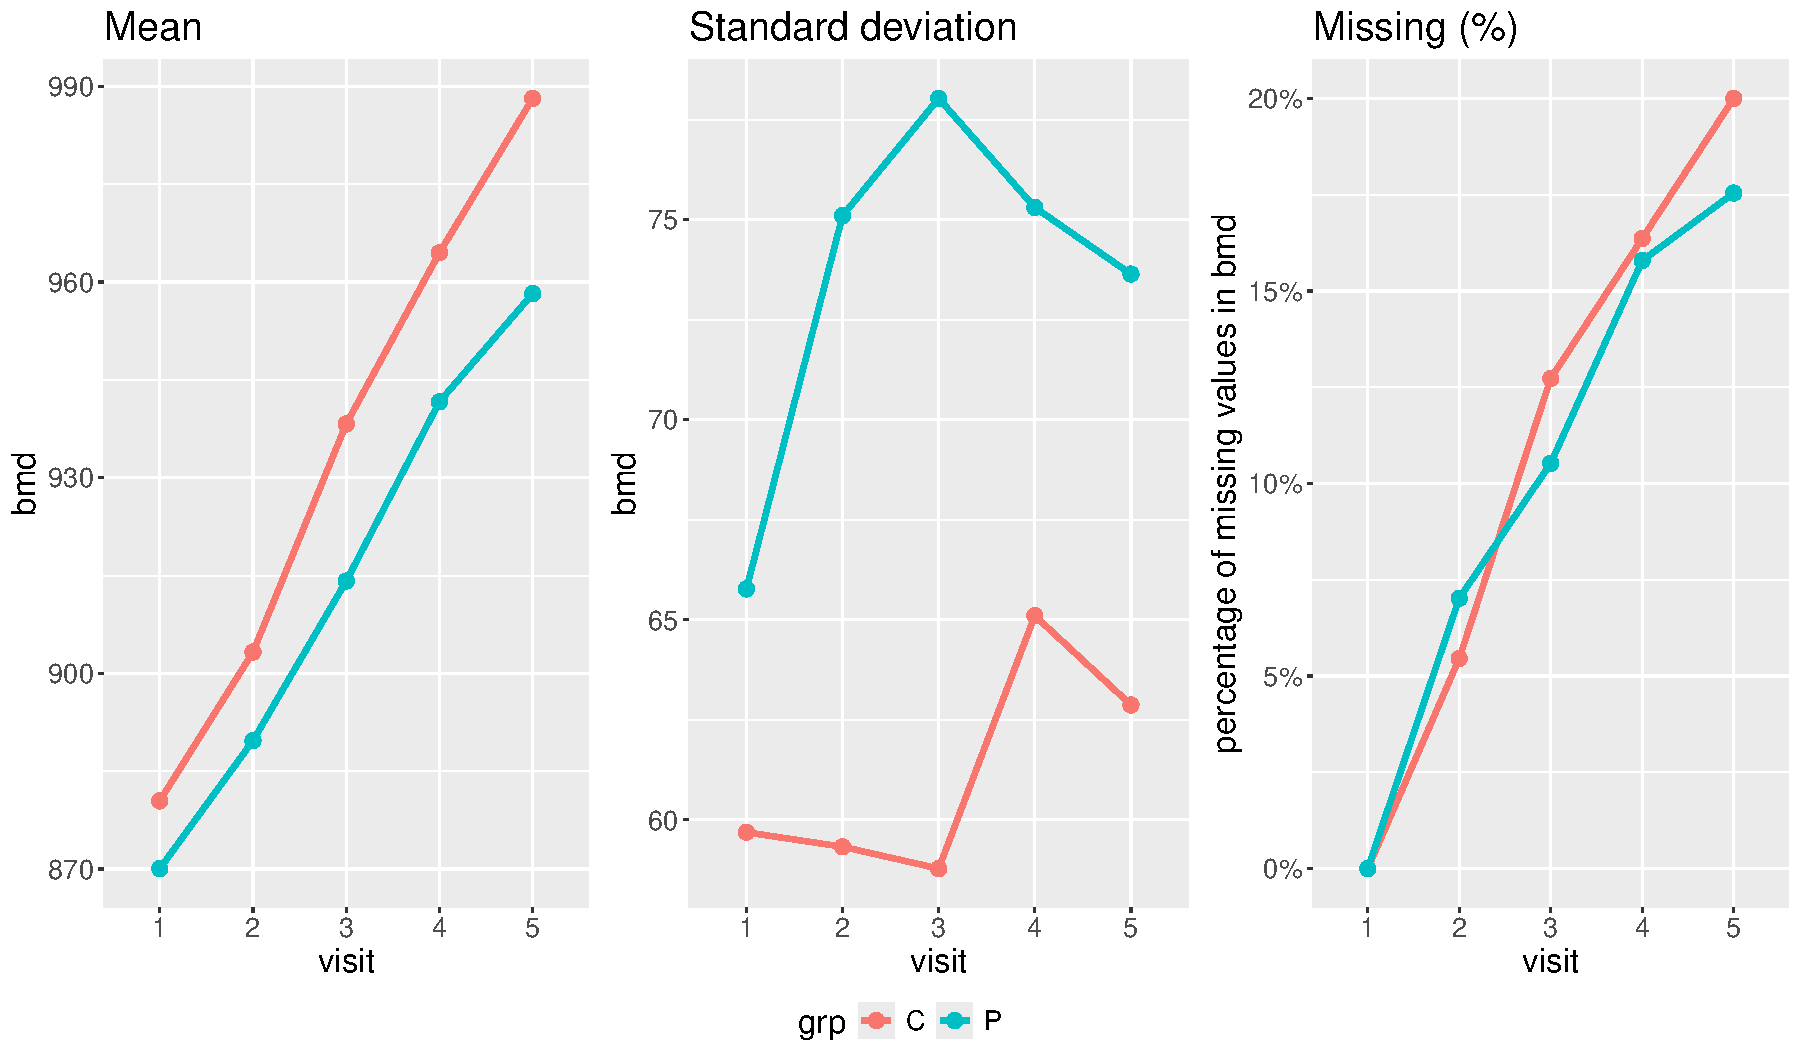
\includegraphics[trim={0 0 0 0},width=1\textwidth]{./figures/summarize.pdf}
\end{center}

\clearpage 
\section{Correlation}
\label{sec:org3e65672}


The \texttt{correlate} function facilitate the estimation of the correlation:
\begin{lstlisting}[language=r,numbers=none]
rrr <- correlate(bmd ~ grp, repetition = ~visit | girl,
                 data = calciumL, use = "pairwise")
rrr
\end{lstlisting}

\phantomsection
\label{}
\begin{verbatim}
Pearson correlation: 
$`grp=C`
           1       2       3       4       5
   1 1.00000 0.95829 0.90808 0.88136 0.85965
   2 0.95829 1.00000 0.95946 0.94590 0.92935
   3 0.90808 0.95946 1.00000 0.97232 0.94427
   4 0.88136 0.94590 0.97232 1.00000 0.96245
   5 0.85965 0.92935 0.94427 0.96245 1.00000

$`grp=P`
           1       2       3       4       5
   1 1.00000 0.97557 0.95640 0.94445 0.91701
   2 0.97557 1.00000 0.97832 0.96333 0.94437
   3 0.95640 0.97832 1.00000 0.98537 0.96597
   4 0.94445 0.96333 0.98537 1.00000 0.98305
   5 0.91701 0.94437 0.96597 0.98305 1.00000
\end{verbatim}

By default Pearson's correlation is computed (argument \texttt{method}). A
graphical representation can be obtained using:
\begin{lstlisting}[language=r,numbers=none]
plot(rrr)
\end{lstlisting}

\begin{center}
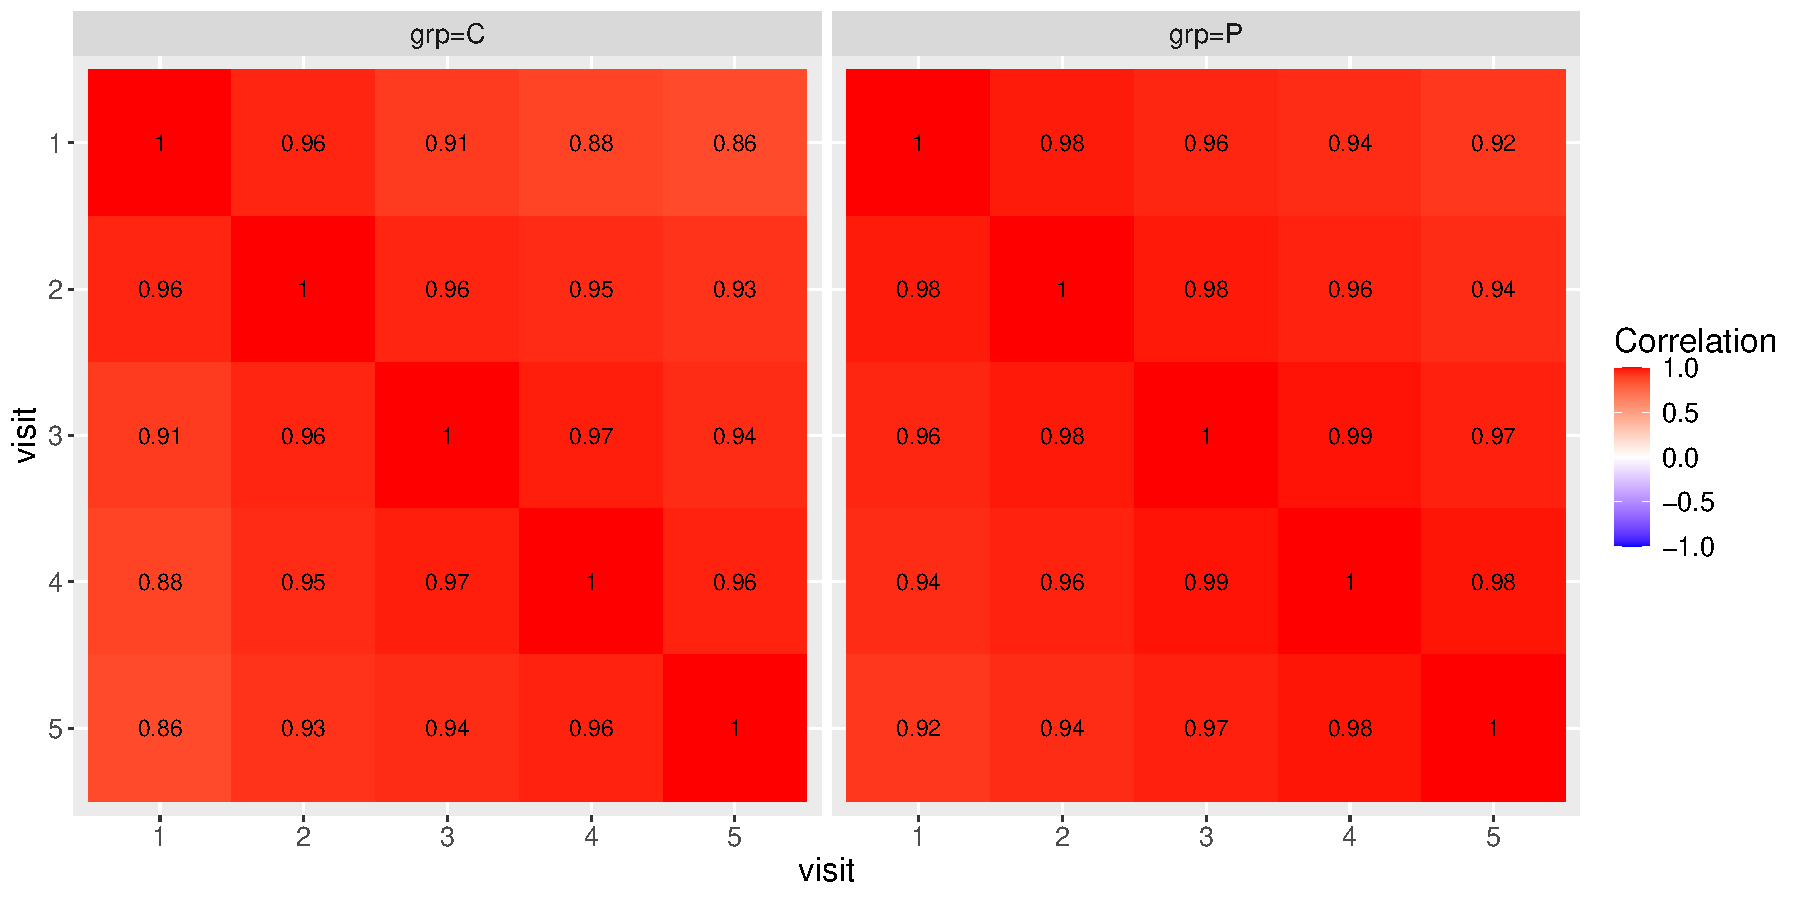
\includegraphics[trim={0 0 0 0},width=1\textwidth]{./figures/correlation.pdf}
\end{center}


\clearpage
\section{Missing data patterns}
\label{sec:orge2faf99}

The \texttt{summarizeNA} function identifies the possible combinations of
observed/missing data:
\begin{lstlisting}[language=r,numbers=none]
mp <- summarizeNA(calciumL, repetition = ~visit | girl)
mp
\end{lstlisting}

\phantomsection
\label{}
\begin{verbatim}
variable frequency missing.pattern n.missing 1 2 3 4 5
      grp       112           00000         0 0 0 0 0 0
  dropout       112           00000         0 0 0 0 0 0
 time.obs        91           00000         0 0 0 0 0 0
                  3           00001         1 0 0 0 0 1
                  5           00011         2 0 0 0 1 1
                  6           00111         3 0 0 1 1 1
                  7           01111         4 0 1 1 1 1
      bmd        91           00000         0 0 0 0 0 0
                  3           00001         1 0 0 0 0 1
                  5           00011         2 0 0 0 1 1
                  6           00111         3 0 0 1 1 1
                  7           01111         4 0 1 1 1 1
\end{verbatim}

A graphical representation can be obtained using \texttt{plot}. Since there
are several variables, one has to specifying the variable relative to
which the missing data pattern should be displayed:
\begin{lstlisting}[language=r,numbers=none]
plot(mp, variable = "bmd")
\end{lstlisting}

See \texttt{help(plot.summarizeNA)} for options to customize the graphical
display.

\begin{center}
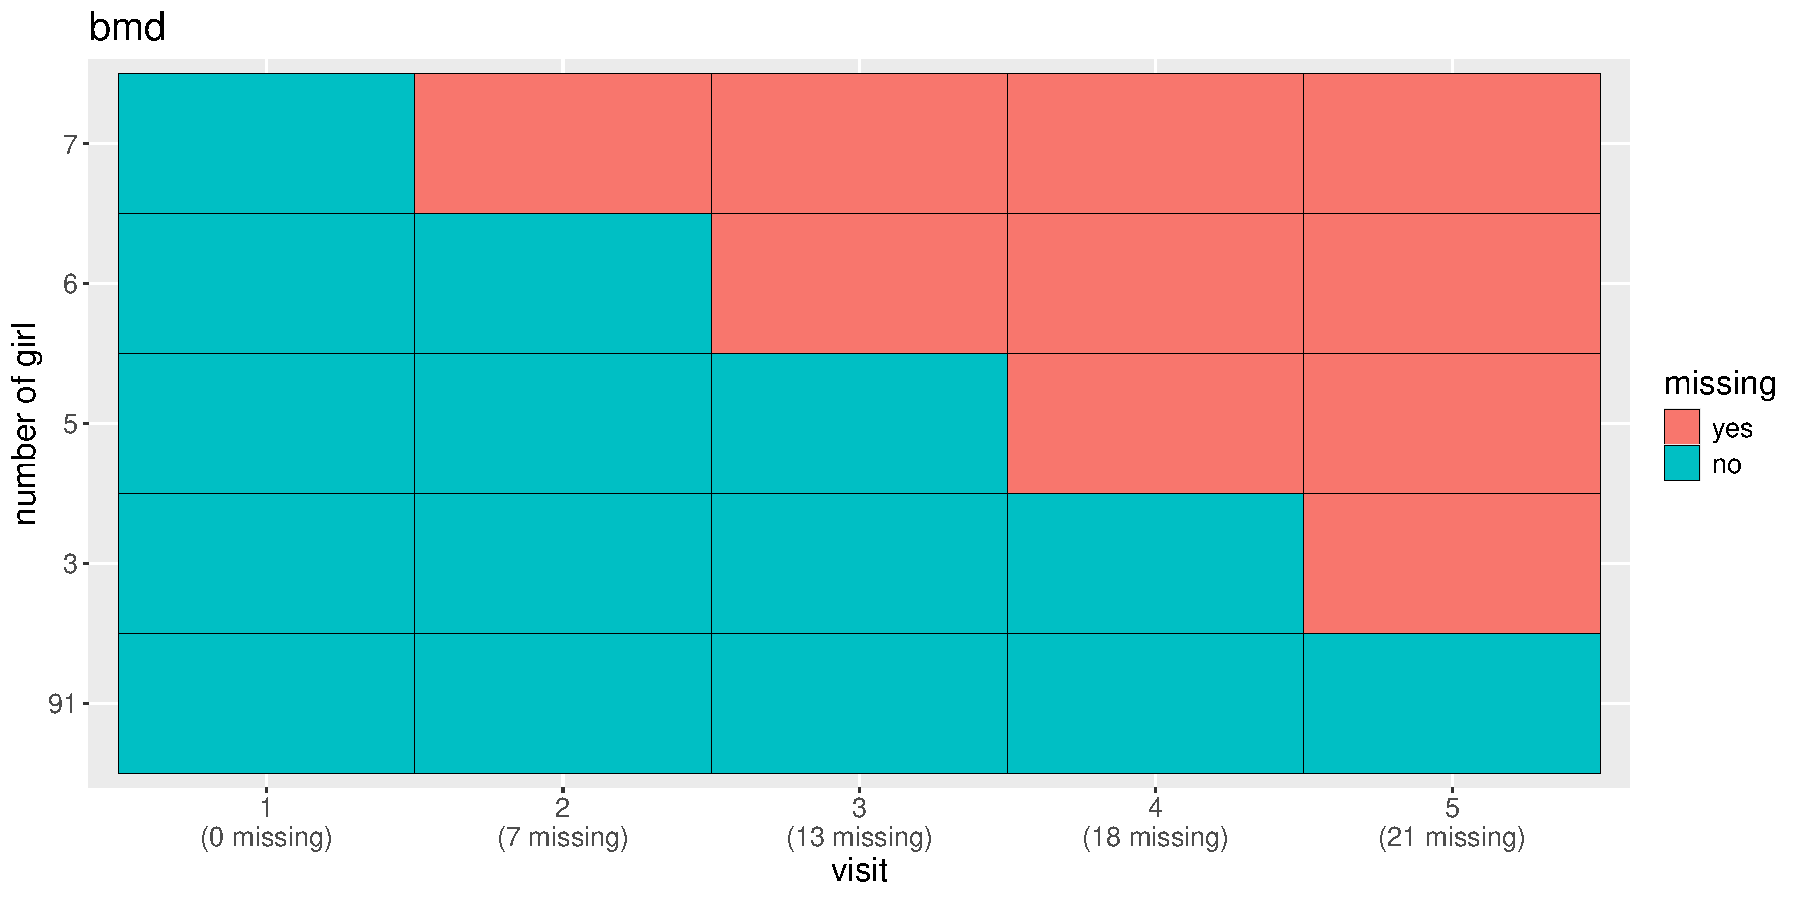
\includegraphics[trim={0 0 0 0},width=1\textwidth]{./figures/summarizeNA.pdf}
\end{center}



\clearpage

A formula should be specified to stratify the missing data pattern per group:
\begin{lstlisting}[language=r,numbers=none]
mpS <- summarizeNA(bmd ~ grp, repetition = ~visit | girl, data = calciumL)
mpS
\end{lstlisting}

\phantomsection
\label{}
\begin{verbatim}
variable grp frequency missing.pattern n.missing 1 2 3 4 5
      bmd   C        44           00000         0 0 0 0 0 0
            C         2           00001         1 0 0 0 0 1
            C         2           00011         2 0 0 0 1 1
            C         4           00111         3 0 0 1 1 1
            C         3           01111         4 0 1 1 1 1
            P        47           00000         0 0 0 0 0 0
            P         1           00001         1 0 0 0 0 1
            P         3           00011         2 0 0 0 1 1
            P         2           00111         3 0 0 1 1 1
            P         4           01111         4 0 1 1 1 1
\end{verbatim}

\begin{lstlisting}[language=r,numbers=none]
plot(mpS, labeller = "label_both")
\end{lstlisting}

\begin{center}
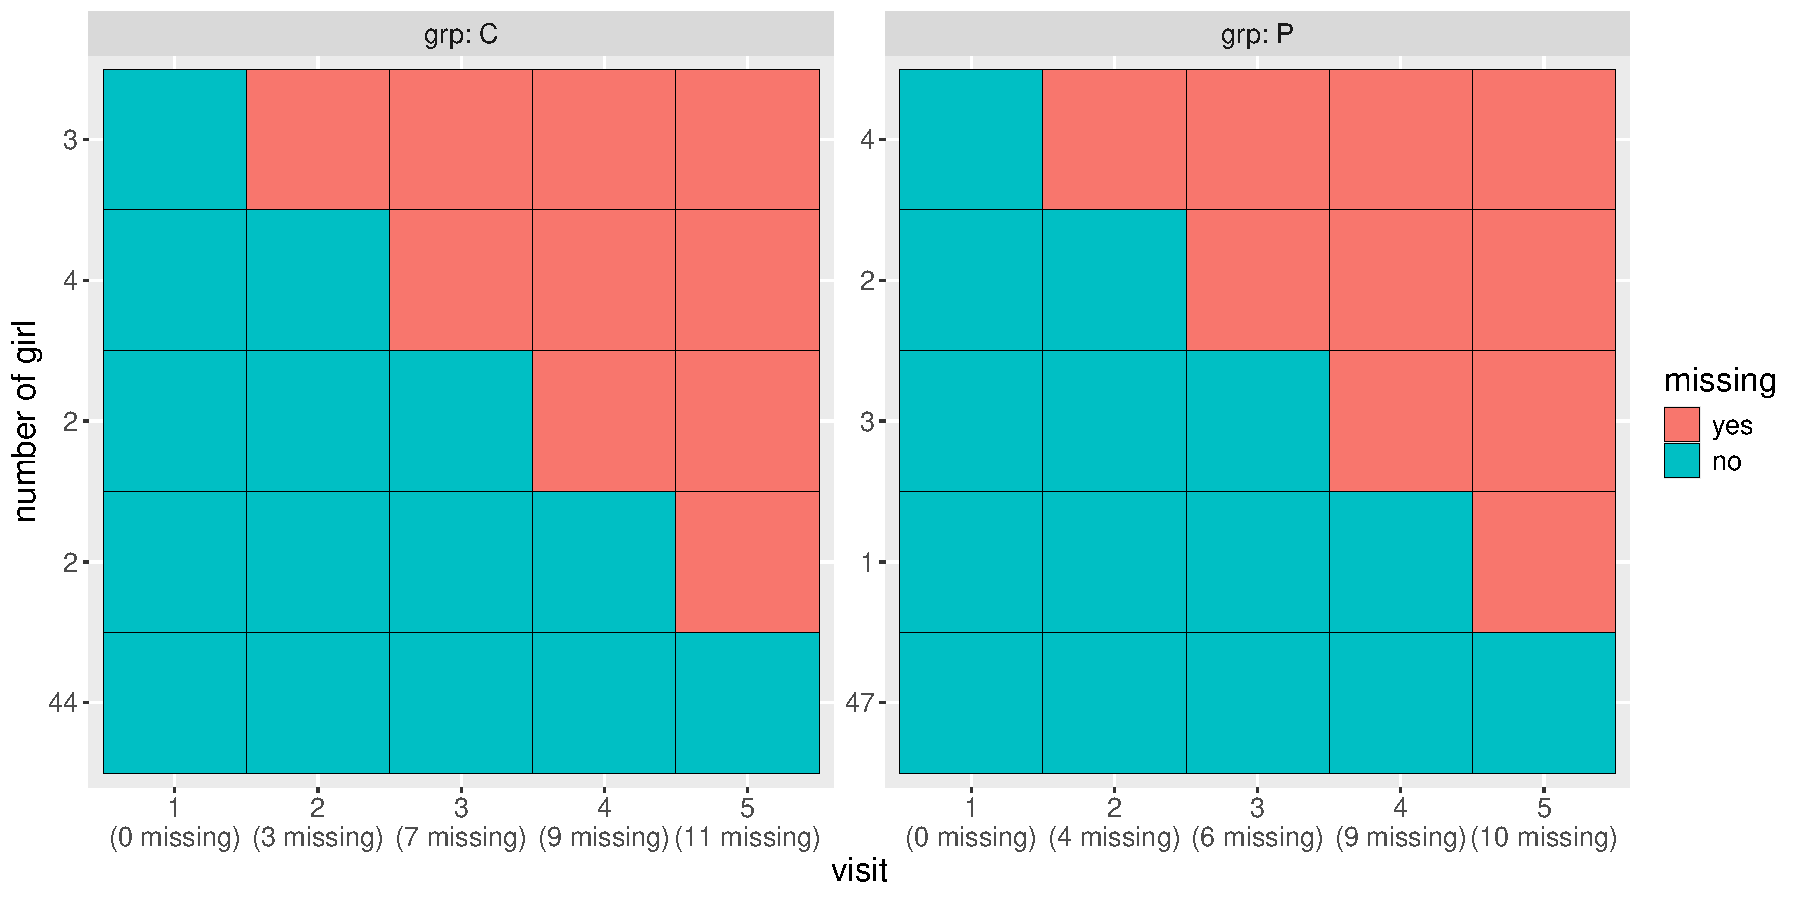
\includegraphics[trim={0 0 0 0},width=1\textwidth]{./figures/summarizeNA-stratified.pdf}
\end{center}



\clearpage
\section{Spaghetti plot}
\label{sec:orgc9cbfa4}

There is (currently) not dedicated function to obtain spaghetti
plots. Instead one can use the ggplot2 package with the long format, e.g.:
\begin{lstlisting}[language=r,numbers=none]
gg.spa <- ggplot(calciumL, aes(x = visit, y = bmd, group = girl, color = grp))
gg.spa <- gg.spa + geom_point() + geom_line()
gg.spa
\end{lstlisting}

\begin{center}
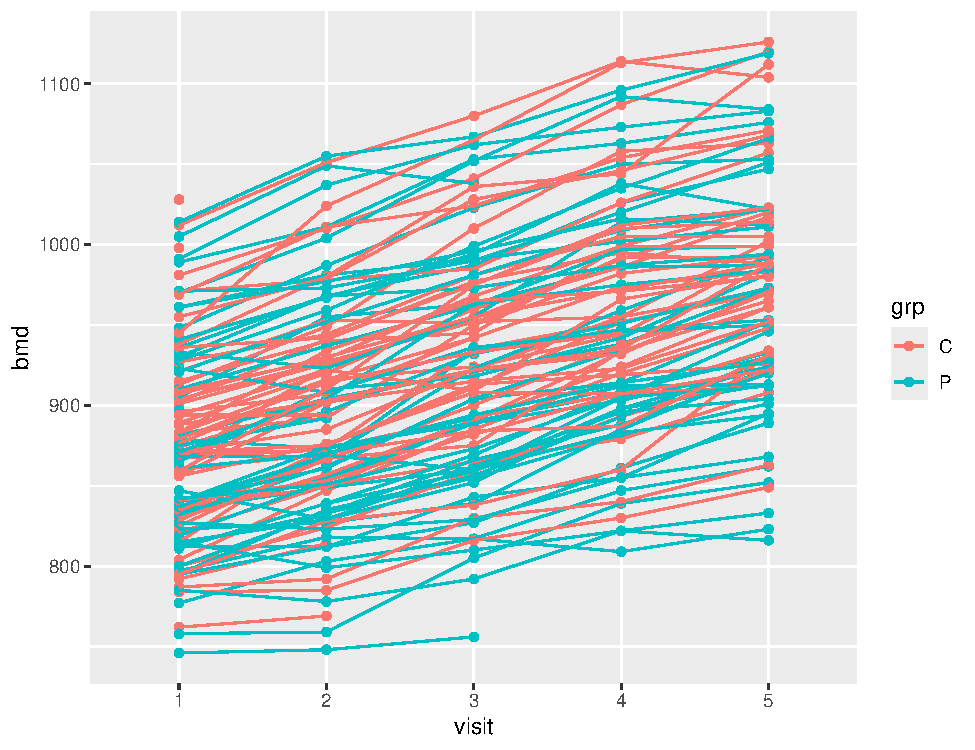
\includegraphics[trim={0 0 0 0},width=1\textwidth]{./figures/spaghetti.pdf}
\end{center}


\clearpage
\section{Scatterplot}
\label{sec:org8a2bfb8}


A scatterplot of the data can obtained by specifying which columns to
display when using the wide format. 
\begin{lstlisting}[language=r,numbers=none]
scatterplot(calciumW, columns = c("bmd1","bmd2","bmd3","bmd4","bmd5")) 
\end{lstlisting}

\begin{center}
\includegraphics[trim={0 0 0 0},width=0.5\textwidth]{./figures/scatterplot-grid2.pdf}
\end{center}

By default and if available, \texttt{scatterplot} will use the \texttt{facet\_grid2}
function from the ggh4x package to combine the different panels of the
graphical display. It outputs a \texttt{ggplot} that can be further
customized:

\begin{lstlisting}[language=r,numbers=none]
gg.sca <- scatterplot(calciumW, columns = c("bmd1","bmd2","bmd3","bmd4","bmd5")) 
class(gg.sca)
gg.sca + theme_minimal() ## right panel
\end{lstlisting}

\begin{center}
\includegraphics[trim={0 0 0 0},width=0.5\textwidth]{./figures/scatterplotMin-grid.pdf}
\end{center}



xxx

\begin{center}
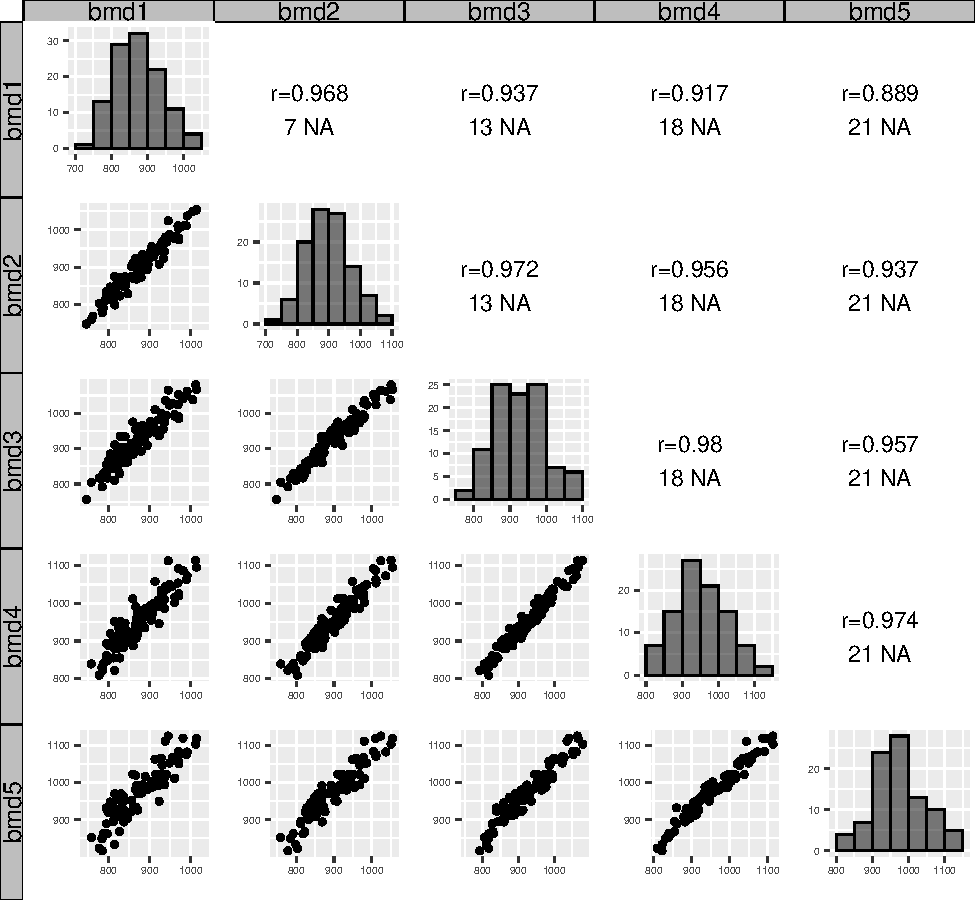
\includegraphics[trim={0 0 0 0},width=\textwidth]{./figures/scatterplot-grid.pdf}
\end{center}


\noindent When using the long format, a formula should describe the
structure of the data: \texttt{outcome \textasciitilde{} order|cluster}
\begin{itemize}
\item the left hand side indicates the values to be displayed (here \texttt{bmd})
\item the right hand side indicates the ordering of the repetitions (here over \texttt{visit}) and
how the repetitions are grouped within clusters (here within \texttt{girl}).
\end{itemize}

When calling \texttt{scatterplot}, the argument \texttt{group} leads to different
color per group and the argument \texttt{type.diag} enables to use histograms
(or density plots) instead of boxplots:
\begin{lstlisting}[language=r,numbers=none]
gg.sca2 <- scatterplot(bmd ~ visit | girl, data = calciumL, ## left panel
                       type.diag = "hist", group = "grp", size.cor = 3)
gg.sca2
\end{lstlisting}


\bigskip

\begin{minipage}{0.48\linewidth}
\begin{center}
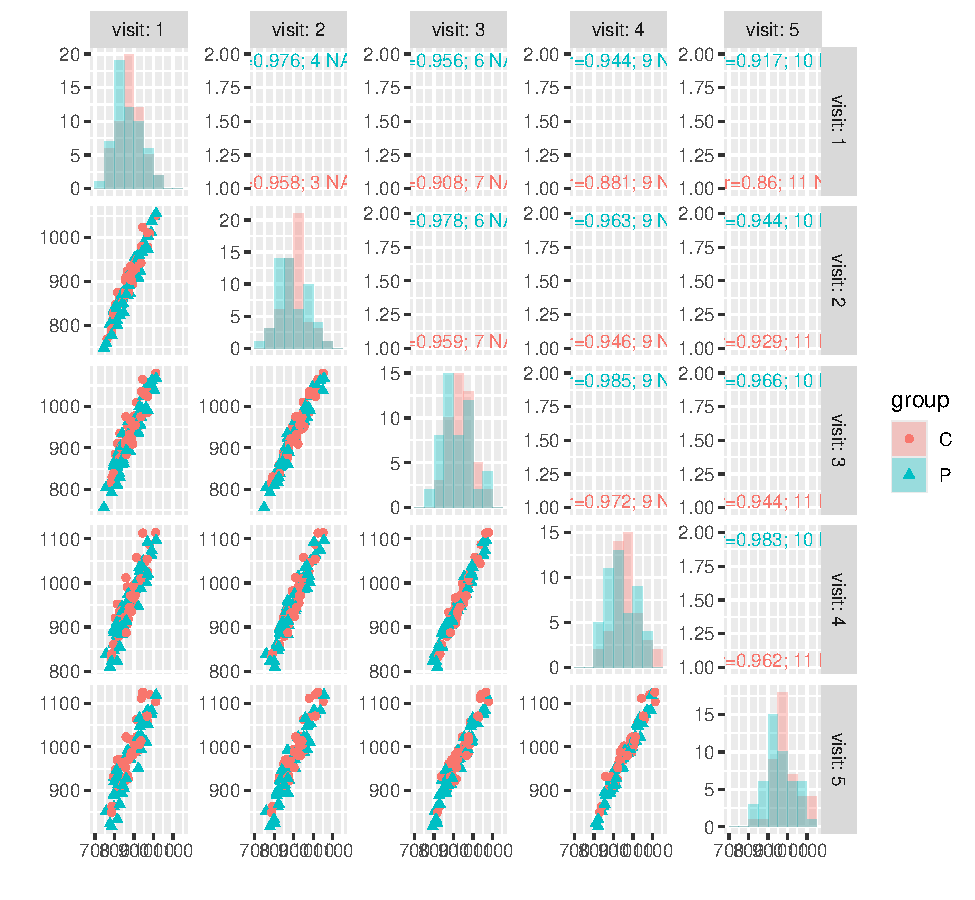
\includegraphics[trim={0 0 0 0},width=\textwidth]{./figures/scatterplot-group.pdf}
\end{center}
\end{minipage}
\begin{minipage}{0.48\linewidth}
\begin{center}
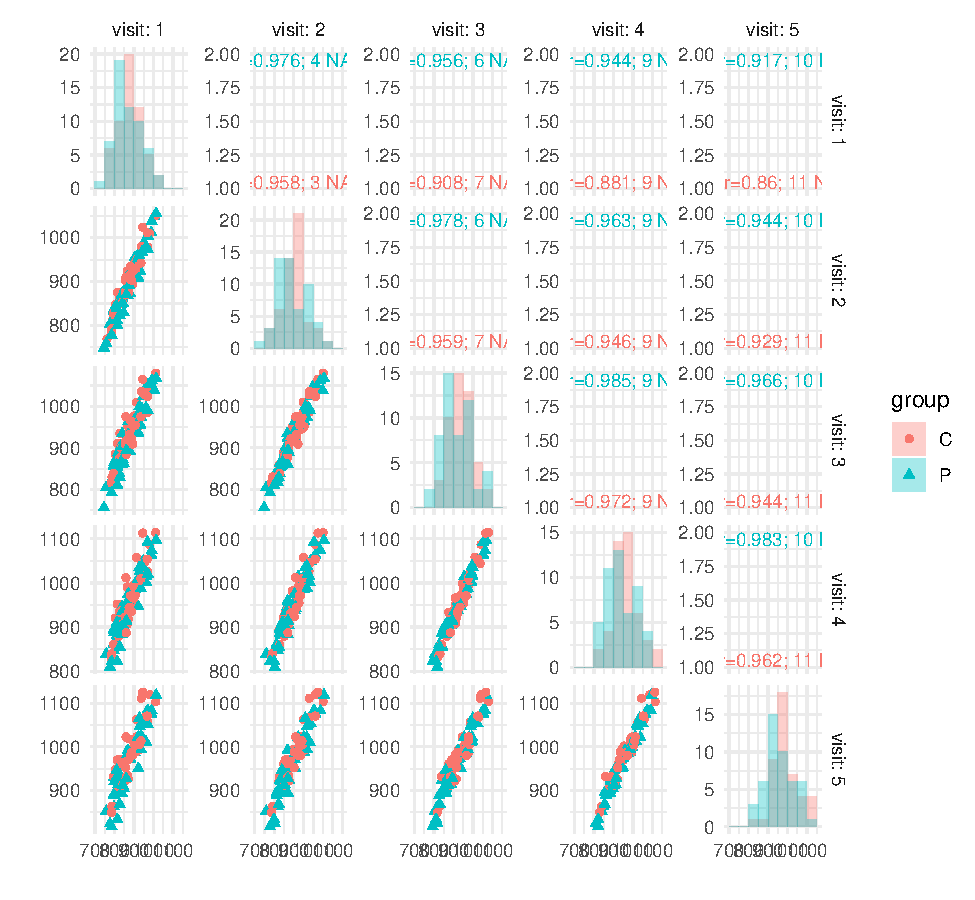
\includegraphics[trim={0 0 0 0},width=\textwidth]{./figures/scatterplotMin-group.pdf}
\end{center}
\end{minipage}


The argument \texttt{size.cor} was used to adjust the font size used when
displaying the estimated correlation and number of missing
values. When the package \texttt{ggh4x} is installed, \texttt{scatterplot} will
output an \texttt{ggplot2} object that can be customized:

\phantomsection
\label{}
\begin{verbatim}
[1] "ggplot2::ggplot" "ggplot"          "ggplot2::gg"     "S7_object"       "gg"
Advarselsbeskeder:
1: Removed 59 rows containing non-finite outside the scale range (`stat_bin()`). 
2: Removed 171 rows containing missing values or values outside the scale range (`geom_point()`).
\end{verbatim}


\bigskip
\end{document}
